\chapter{Ricerca completa}

La \key{ricerca completa} (o esaustiva)
è un metodo generale che può essere utilizzato 
per risolvere quasi qualsiasi problema.
L'idea è di generare tutte le soluzioni
possibili per il problema con un approcio a forza bruta,
e poi selezionare la migliore soluzione possibile
oppure contare il numero di soluzioni, a seconda
di quello che richiede il problema.

La ricerca completa è una buona tecnica
se il tempo è sufficiente per generare tutte le soluzioni,
perchè in generale è facile da implementare
e da sempre la risposta corretta.
Se la ricerca completa è troppo lenta,
può essere bisogno utilizzare altre tecniche, 
come gli algoritmi greedy o la programmazione dinamica.

\section{Generazioni di sottoinsiemi}

\index{sottoinsiemi}

Si considera come prima cosa il problema di 
generare tutti i sottoinsiemi possibili di 
un insieme di $n$ elementi.
Per esempio, i sottoinsiemi di $\{0,1,2\}$ sono
$\emptyset$, $\{0\}$, $\{1\}$, $\{2\}$, $\{0,1\}$,
$\{0,2\}$, $\{1,2\}$ e $\{0,1,2\}$.
I due tipici metodi per generare sottoinsiemi prevedono
o che si faccia una ricerca ricorsiva oppure
che si sfrutti la rappresentazione binaria degli interi.

\subsubsection{Metodo 1}

Un modo elegante per generare tutti i sottoinsiemi 
di un insieme dato è quello che usa la ricorsione.
La seguente funzione \texttt{search}
genera i sottoinsiemi dell'insieme
$\{0,1,\ldots,n-1\}$.
La funzione contieme un vettore \texttt{subset}
che conterrà gli elementi di ogni sottoinsieme.
La ricerca inizia quando viene chiamata la funzione
passandogli come parametro il valore 0.

\begin{lstlisting}
void search(int k) {
    if (k == n) {
        // processa il sottoinsieme
    } else {
        search(k+1);
        subset.push_back(k);
        search(k+1);
        subset.pop_back();
    }
}
\end{lstlisting}

Quando la funzione \texttt{search}
viene chiamata con il parametro $k$,
decide se includere o meno l'elemento $k$
nel sottoinsieme, e, in entrambi i casi,
richiama se stessa con il parametro $k+1$.
Comunque, se $k=n$, 
la funzione si accorge che tutti gli elementi sono stati processati e
viene generato il sottoinsieme.

Il seguente albero mostra le chiamate ricorsive della funzione con $n=3$.
Si può vedere come è sempre possibile scegliere o il ramo sinistro
($k$ non è incluso nel sottoinsieme) o il ramo destro
($k$ è incluso nel sottoinsieme).

\begin{center}
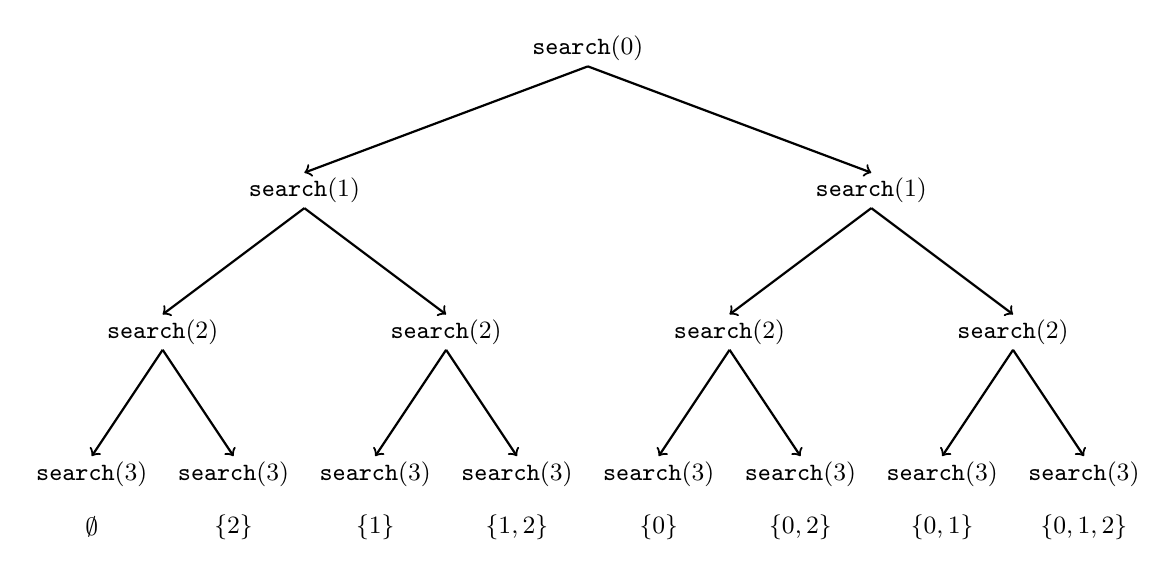
\begin{tikzpicture}[scale=.45]
  \begin{scope}
    \small
    \node at (0,0) {$\texttt{search}(0)$};

    \node at (-8,-4) {$\texttt{search}(1)$};
    \node at (8,-4) {$\texttt{search}(1)$};

    \path[draw,thick,->] (0,0-0.5) -- (-8,-4+0.5);
    \path[draw,thick,->] (0,0-0.5) -- (8,-4+0.5);

    \node at (-12,-8) {$\texttt{search}(2)$};
    \node at (-4,-8) {$\texttt{search}(2)$};
    \node at (4,-8) {$\texttt{search}(2)$};
    \node at (12,-8) {$\texttt{search}(2)$};

    \path[draw,thick,->] (-8,-4-0.5) -- (-12,-8+0.5);
    \path[draw,thick,->] (-8,-4-0.5) -- (-4,-8+0.5);
    \path[draw,thick,->] (8,-4-0.5) -- (4,-8+0.5);
    \path[draw,thick,->] (8,-4-0.5) -- (12,-8+0.5);

    \node at (-14,-12) {$\texttt{search}(3)$};
    \node at (-10,-12) {$\texttt{search}(3)$};
    \node at (-6,-12) {$\texttt{search}(3)$};
    \node at (-2,-12) {$\texttt{search}(3)$};
    \node at (2,-12) {$\texttt{search}(3)$};
    \node at (6,-12) {$\texttt{search}(3)$};
    \node at (10,-12) {$\texttt{search}(3)$};
    \node at (14,-12) {$\texttt{search}(3)$};

    \node at (-14,-13.5) {$\emptyset$};
    \node at (-10,-13.5) {$\{2\}$};
    \node at (-6,-13.5) {$\{1\}$};
    \node at (-2,-13.5) {$\{1,2\}$};
    \node at (2,-13.5) {$\{0\}$};
    \node at (6,-13.5) {$\{0,2\}$};
    \node at (10,-13.5) {$\{0,1\}$};
    \node at (14,-13.5) {$\{0,1,2\}$};


    \path[draw,thick,->] (-12,-8-0.5) -- (-14,-12+0.5);
    \path[draw,thick,->] (-12,-8-0.5) -- (-10,-12+0.5);
    \path[draw,thick,->] (-4,-8-0.5) -- (-6,-12+0.5);
    \path[draw,thick,->] (-4,-8-0.5) -- (-2,-12+0.5);
    \path[draw,thick,->] (4,-8-0.5) -- (2,-12+0.5);
    \path[draw,thick,->] (4,-8-0.5) -- (6,-12+0.5);
    \path[draw,thick,->] (12,-8-0.5) -- (10,-12+0.5);
    \path[draw,thick,->] (12,-8-0.5) -- (14,-12+0.5);
\end{scope}
\end{tikzpicture}
\end{center}

\subsubsection{Metodo 2}

Un altro modo di generare dei sottoinsiemi è basato
sulla rapprensentazione binaria degli interi.
Ogni sottoinsieme di un insieme di $n$ elementi
può essere rappresentato come una sequenza di $n$ bit,
che corrisponde a un intero tra $0 \ldots 2^n-1$.
Gli uno nella sequenza indicano quali elementi
sono inclusi nel sottoinsieme.

La rappresentazione usuale prevede che l'ultimo bit corrisponda
all'elemento 0, il penultimo bit all'elemento 1 e così via.
Per esempio, la rappresentazione di 25 è 11001, che corrisponde al sottoinsieme
$\{0,3,4\}$.
Il seguente codice scorre tutti i sottoinsiemi di un 
insieme di $n$ elementi

\begin{lstlisting}
for (int b = 0; b < (1<<n); b++) {
    // processa il sottoinsieme
}
\end{lstlisting}

Il seguente codice mostra come sia possibile trovare gli
elementi di un sottoinsieme che corrisponde a una sequenza di bit.
Quando ogni sottoinsieme viene processato,
il codice costruisce un vettore che contiene gli
elementi del sottoinsieme.

\begin{lstlisting}
for (int b = 0; b < (1<<n); b++) {
    vector<int> subset;
    for (int i = 0; i < n; i++) {
        if (b&(1<<i)) subset.push_back(i);
    }
}
\end{lstlisting}

\section{Generazione delle permutazioni}

\index{permutazioni}

Un altro problema è quello di generare tutte le combinazioni possibili
di un insieme di $n$ elementi.
Per esempio, le permutazioni di $\{0,1,2\}$ sono
$(0,1,2)$, $(0,2,1)$, $(1,0,2)$, $(1,2,0)$,
$(2,0,1)$ e $(2,1,0)$.
Anche in questo caso si possono seguire due strade:
o usare la ricorsione oppure creare tutte le permutazioni in 
modo iterativo.

\subsubsection{Metodo 1}

Come per i sottoinsiemi, le permutazioni possono
essere generate con la ricorsione.
La funzione \texttt{search} produce tutte le 
permutazioni dell'insieme $\{0,1,\ldots,n-1\}$.
La funzione costruisce il vettore \texttt{permutation}
che contiene la permutazione,
e la ricerca inizia con la funzione che viene chiamata
senza parametri.

\begin{lstlisting}
void search() {
    if (permutation.size() == n) {
        // processa la permutazione
    } else {
        for (int i = 0; i < n; i++) {
            if (chosen[i]) continue;
            chosen[i] = true;
            permutation.push_back(i);
            search();
            chosen[i] = false;
            permutation.pop_back();
        }
    }
}
\end{lstlisting}

Ogni chiamata di funzione aggiunge un nuovo elemento
a \texttt{permutation}.
L'array \texttt{chosen} indica quali elementi sono stati già aggiunti nella permutazione.
Se la dimensione di \texttt{permutation} è uguale alla dimensione dell'insieme,
allora è stata generata una nuova permutazione.

\subsubsection{Metodo 2}

\index{next\_permutation@\texttt{next\_permutation}}

Un altro metodo per generare una permutazione
è di iniziare con la permutazione
$\{0,1,\ldots,n-1\}$ e utilizzare ripetutamente una funzione che costruisce
la prossima permutazione in ordine crescente.
La libreria standard del C++ contiene la funzione
\texttt{next\_permutation} che fa proprio questo:

\begin{lstlisting}
vector<int> permutation;
for (int i = 0; i < n; i++) {
    permutation.push_back(i);
}
do {
    // processa la permutazione
} while (next_permutation(permutation.begin(),permutation.end()));
\end{lstlisting}

\section{Backtracking}

\index{backtracking}

Un algoritmo di \key{backtracking} 
inizia con la soluzione vuota e la estende
passo dopo passo.
Ricorsivamente vengono creati tutti 
i differenti modi in cui può essere
costruita una soluzione.

\index{problema delle regine}

Si consideri come esempio il problema
di calcolare il numero di modi
in cui $n$ regine possono essere piazzate
su una scacchiera $n \times n$ in modo che
nessuna regina ne attacchi un'altra.
Per esempio, quando $n=4$,
ci sono due soluzioni possibili:

\begin{center}
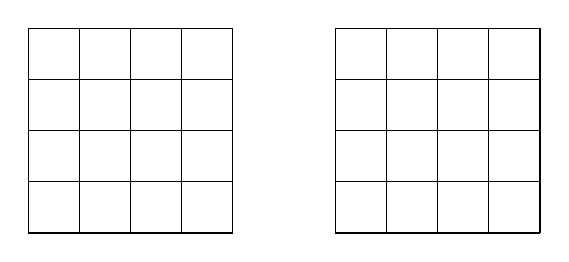
\begin{tikzpicture}[scale=.65]
  \begin{scope}
    \draw (0, 0) grid (4, 4);
    \node at (1.5,3.5) {\symqueen};
    \node at (3.5,2.5) {\symqueen};
    \node at (0.5,1.5) {\symqueen};
    \node at (2.5,0.5) {\symqueen};

    \draw (6, 0) grid (10, 4);
    \node at (6+2.5,3.5) {\symqueen};
    \node at (6+0.5,2.5) {\symqueen};
    \node at (6+3.5,1.5) {\symqueen};
    \node at (6+1.5,0.5) {\symqueen};

  \end{scope}
\end{tikzpicture}
\end{center}

Il problema può essere risolto utilizzando il backtracking
e piazzando le regine sulla scacchiera riga per riga.
Più precisamente verrà piazzata una regina in ogni riga 
in modo che nessuna regina attacchi una di quelle piazzate in precedenza.
Viene trovata una soluzione quando 
$n$ regine sono state inserite sulla scacchiera.

Per esempio con $n=4$,
alcune soluzioni parziali generate con il backtracking
sono le seguenti:

\begin{center}
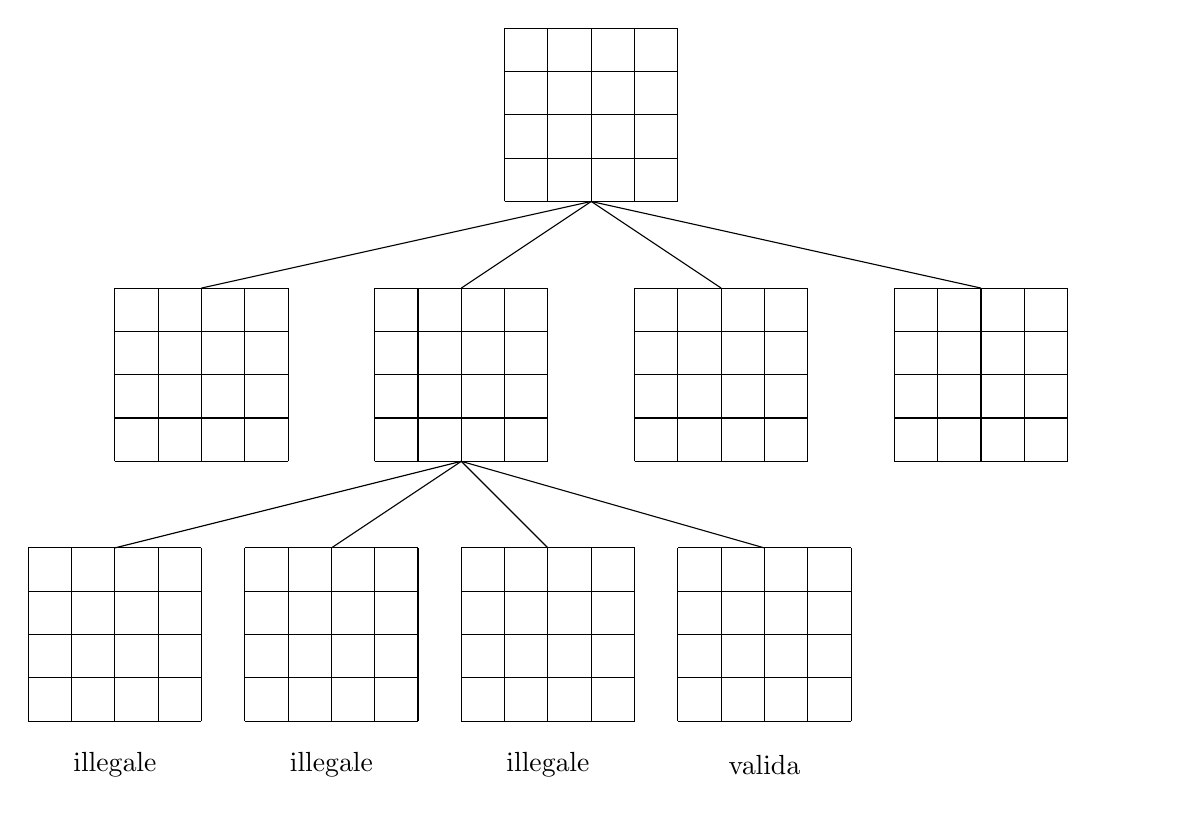
\begin{tikzpicture}[scale=.55]
  \begin{scope}
    \draw (0, 0) grid (4, 4);

    \draw (-9, -6) grid (-5, -2);
    \draw (-3, -6) grid (1, -2);
    \draw (3, -6) grid (7, -2);
    \draw (9, -6) grid (13, -2);

    \node at (-9+0.5,-3+0.5) {\symqueen};
    \node at (-3+1+0.5,-3+0.5) {\symqueen};
    \node at (3+2+0.5,-3+0.5) {\symqueen};
    \node at (9+3+0.5,-3+0.5) {\symqueen};

    \draw (2,0) -- (-7,-2);
    \draw (2,0) -- (-1,-2);
    \draw (2,0) -- (5,-2);
    \draw (2,0) -- (11,-2);

    \draw (-11, -12) grid (-7, -8);
    \draw (-6, -12) grid (-2, -8);
    \draw (-1, -12) grid (3, -8);
    \draw (4, -12) grid (8, -8);
    \draw[white] (11, -12) grid (15, -8);
    \node at (-11+1+0.5,-9+0.5) {\symqueen};
    \node at (-6+1+0.5,-9+0.5) {\symqueen};
    \node at (-1+1+0.5,-9+0.5) {\symqueen};
    \node at (4+1+0.5,-9+0.5) {\symqueen};
    \node at (-11+0+0.5,-10+0.5) {\symqueen};
    \node at (-6+1+0.5,-10+0.5) {\symqueen};
    \node at (-1+2+0.5,-10+0.5) {\symqueen};
    \node at (4+3+0.5,-10+0.5) {\symqueen};

    \draw (-1,-6) -- (-9,-8);
    \draw (-1,-6) -- (-4,-8);
    \draw (-1,-6) -- (1,-8);
    \draw (-1,-6) -- (6,-8);

    \node at (-9,-13) {illegale};
    \node at (-4,-13) {illegale};
    \node at (1,-13) {illegale};
    \node at (6,-13) {valida};

  \end{scope}
\end{tikzpicture}
\end{center}

Al livello finale, le prime tre configurazioni sono illegali,
perchè le regine si attaccano tra di loro.
Invece la quarta configurazione è valida e può essere estesa
per arrivare a una soluzione completa aggiungendo altre
due regine alla scacchiera.

C'è solo un modo per piazzare le due ultime regine sulla scacchiera.

\begin{samepage}
L'algoritmo può essere scritto come segue:
\begin{lstlisting}
void search(int y) {
    if (y == n) {
        count++;
        return;
    }
    for (int x = 0; x < n; x++) {
        if (column[x] || diag1[x+y] || diag2[x-y+n-1]) continue;
        column[x] = diag1[x+y] = diag2[x-y+n-1] = 1;
        search(y+1);
        column[x] = diag1[x+y] = diag2[x-y+n-1] = 0;
    }
}
\end{lstlisting}
\end{samepage}

La ricerca inizia chiamando \texttt{search(0)}.
La dimensione della scacchiera è $n$,
e il codice memorizza il numero di soluzioni in \texttt{count}.

Il codice assume che le righe e le colonne 
della scacchiera siano numerate da 0 a $n-1$.
Quando la funzione \texttt{search} viene chiamata
con il parametro $y$,
inserisce una regina nella riga $y$
e poi richiama se stessa con il parametro $y+1$.
Se $y=n$ è stata trovata una soluzione
e la variabile \texttt{count} viene incrementata di uno.

L'array \texttt{column} tiene traccia delle colonne che contengono una regina,
e gli array \texttt{diag1} e \texttt{diag2}
tengono traccia delle diagonali.
Non può essere aggiunta un'altra regina a una 
colonna o a una diagonale che già contiene una regina.
Per esempio, le colonne e le diagonali di una
scacchiera $4 \times 4$ sono numerate come segue:

\begin{center}
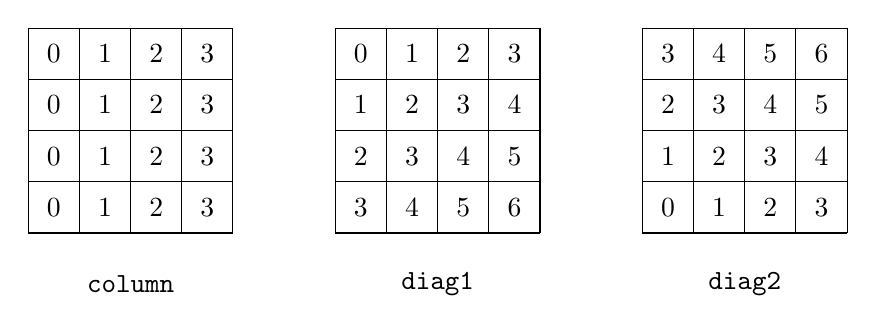
\begin{tikzpicture}[scale=.65]
  \begin{scope}
    \draw (0-6, 0) grid (4-6, 4);
    \node at (-6+0.5,3.5) {$0$};
    \node at (-6+1.5,3.5) {$1$};
    \node at (-6+2.5,3.5) {$2$};
    \node at (-6+3.5,3.5) {$3$};
    \node at (-6+0.5,2.5) {$0$};
    \node at (-6+1.5,2.5) {$1$};
    \node at (-6+2.5,2.5) {$2$};
    \node at (-6+3.5,2.5) {$3$};
    \node at (-6+0.5,1.5) {$0$};
    \node at (-6+1.5,1.5) {$1$};
    \node at (-6+2.5,1.5) {$2$};
    \node at (-6+3.5,1.5) {$3$};
    \node at (-6+0.5,0.5) {$0$};
    \node at (-6+1.5,0.5) {$1$};
    \node at (-6+2.5,0.5) {$2$};
    \node at (-6+3.5,0.5) {$3$};

    \draw (0, 0) grid (4, 4);
    \node at (0.5,3.5) {$0$};
    \node at (1.5,3.5) {$1$};
    \node at (2.5,3.5) {$2$};
    \node at (3.5,3.5) {$3$};
    \node at (0.5,2.5) {$1$};
    \node at (1.5,2.5) {$2$};
    \node at (2.5,2.5) {$3$};
    \node at (3.5,2.5) {$4$};
    \node at (0.5,1.5) {$2$};
    \node at (1.5,1.5) {$3$};
    \node at (2.5,1.5) {$4$};
    \node at (3.5,1.5) {$5$};
    \node at (0.5,0.5) {$3$};
    \node at (1.5,0.5) {$4$};
    \node at (2.5,0.5) {$5$};
    \node at (3.5,0.5) {$6$};

    \draw (6, 0) grid (10, 4);
    \node at (6.5,3.5) {$3$};
    \node at (7.5,3.5) {$4$};
    \node at (8.5,3.5) {$5$};
    \node at (9.5,3.5) {$6$};
    \node at (6.5,2.5) {$2$};
    \node at (7.5,2.5) {$3$};
    \node at (8.5,2.5) {$4$};
    \node at (9.5,2.5) {$5$};
    \node at (6.5,1.5) {$1$};
    \node at (7.5,1.5) {$2$};
    \node at (8.5,1.5) {$3$};
    \node at (9.5,1.5) {$4$};
    \node at (6.5,0.5) {$0$};
    \node at (7.5,0.5) {$1$};
    \node at (8.5,0.5) {$2$};
    \node at (9.5,0.5) {$3$};

    \node at (-4,-1) {\texttt{column}};
    \node at (2,-1) {\texttt{diag1}};
    \node at (8,-1) {\texttt{diag2}};

  \end{scope}
\end{tikzpicture}
\end{center}

Sia $q(n)$ il numero di modi con cui possono
essere piazzate $n$ regine su una scacchiera $n \times n$.
Il precedente algoritmo fornisce come soluzione,
ad esempio nel caso $8 \times 8$, $q(8)=92$.
Quando $n$ aumenta, la ricerca diventa velocemente molto lenta,
perchè il numero di soluzioni cresce esponenzialmente.
Per esempio questo algoritmo impiega circa un minuto per
calcolare $q(16)=14772512$ su un computer moderno\footnote{
Non esiste un modo efficiente per calcolare valori grandi di $q(n)$. 
Il record attuale è $q(27)=234907967154122528$, calcolato nel 2016 \cite{q27}.}.

\section{\textit{Pruning} dell'albero di ricerca}

Il backtracking può essere spesso ottimizzato 
potando (\textit{pruning} in inglese) l'albero di ricerca.
L'idea di base è di aggiungere 
''intelligenza'' all'algoritmo
in modo che possa notare quanto prima se una
soluzione parziale può essere estesa fino ad arrivare
a una soluzione completa oppure no.
Questo tipo di ottimizzazione può migliorare
enormemente l'efficienza della ricerca.

Si consideri ad esempio il problema di calcolare
il numero di percorsi in una griglia
$n \times n$ che vanno dall'angolo superiore sinistro 
all'angolo in basso a destra in modo tale che
ogni percorso visiti tutti i quadrati una e una sola volta.
Per esempio in una griglia $7 \times 7$,
ci sono 111712 di tali percorsi.
Uno dei percorsi è quello che segue:

\begin{center}
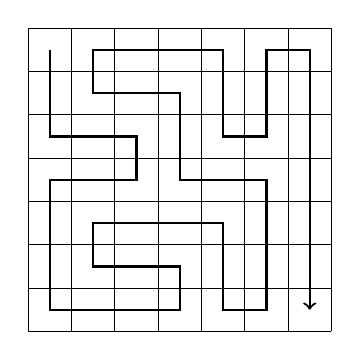
\begin{tikzpicture}[scale=.55]
  \begin{scope}
    \draw (0, 0) grid (7, 7);
    \draw[thick,->] (0.5,6.5) -- (0.5,4.5) -- (2.5,4.5) --
          (2.5,3.5) -- (0.5,3.5) -- (0.5,0.5) --
          (3.5,0.5) -- (3.5,1.5) -- (1.5,1.5) --
          (1.5,2.5) -- (4.5,2.5) -- (4.5,0.5) --
          (5.5,0.5) -- (5.5,3.5) -- (3.5,3.5) --
          (3.5,5.5) -- (1.5,5.5) -- (1.5,6.5) --
          (4.5,6.5) -- (4.5,4.5) -- (5.5,4.5) --
          (5.5,6.5) -- (6.5,6.5) -- (6.5,0.5);
  \end{scope}
\end{tikzpicture}
\end{center}

Ci si concentrerà adesso su questo esempio perchè
è di una difficoltà appropriata per dimostrare il funzionamento
dell'idea.
Partendo dall'algoritmo di backtracking diretto,
verranno successivamente mostrati dei miglioramenti
ottenuti applicando via via osservazioni diverse che
porteranno a una potatura dell'albero di ricerca.
Dopo ogni ottimizzazione verranno misurati il tempo di 
esecuzione e il numero di chiamate ricorsive e si vedrà chiaramente
l'effetto di ogni ottimizzazione sull'efficienza complessiva
della ricerca.

\subsubsection{Algoritmo diretto}

La prima versione dell'algoritmo non contiene nessuna ottimizzazione.
Il baktracking genererà tutti i percorsi possibili dall'angolo in alto
a sinistra a quello in basso a destra e li conterà.

\begin{itemize}
\item
tempo di esecuzione: 483 secondi
\item
numero di chiamate ricorsive: 76 miliardi
\end{itemize}

\subsubsection{Ottimizzazione 1}

All'interno di una qualsiasi soluzione la prima mossa
o è verso il basso oppure verso destra. Inoltre ci sono sempre
due percorsi che sono simmetrici rispetto alla diagonale 
della griglia dopo aver effettuato il primo passo.
Per esempio i seguenti percorsi sono simmetrici:

\begin{center}
\begin{tabular}{ccc}
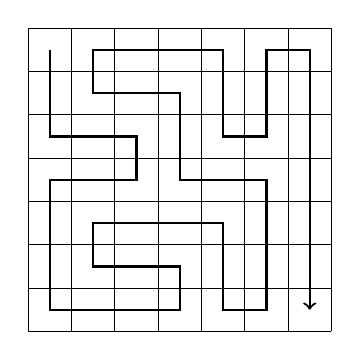
\begin{tikzpicture}[scale=.55]
  \begin{scope}
    \draw (0, 0) grid (7, 7);
    \draw[thick,->] (0.5,6.5) -- (0.5,4.5) -- (2.5,4.5) --
          (2.5,3.5) -- (0.5,3.5) -- (0.5,0.5) --
          (3.5,0.5) -- (3.5,1.5) -- (1.5,1.5) --
          (1.5,2.5) -- (4.5,2.5) -- (4.5,0.5) --
          (5.5,0.5) -- (5.5,3.5) -- (3.5,3.5) --
          (3.5,5.5) -- (1.5,5.5) -- (1.5,6.5) --
          (4.5,6.5) -- (4.5,4.5) -- (5.5,4.5) --
          (5.5,6.5) -- (6.5,6.5) -- (6.5,0.5);
  \end{scope}
\end{tikzpicture}
& \hspace{20px}
& 
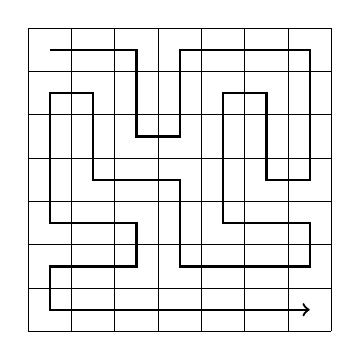
\begin{tikzpicture}[scale=.55]
  \begin{scope}[yscale=1,xscale=-1,rotate=-90]
    \draw (0, 0) grid (7, 7);
    \draw[thick,->] (0.5,6.5) -- (0.5,4.5) -- (2.5,4.5) --
          (2.5,3.5) -- (0.5,3.5) -- (0.5,0.5) --
          (3.5,0.5) -- (3.5,1.5) -- (1.5,1.5) --
          (1.5,2.5) -- (4.5,2.5) -- (4.5,0.5) --
          (5.5,0.5) -- (5.5,3.5) -- (3.5,3.5) --
          (3.5,5.5) -- (1.5,5.5) -- (1.5,6.5) --
          (4.5,6.5) -- (4.5,4.5) -- (5.5,4.5) --
          (5.5,6.5) -- (6.5,6.5) -- (6.5,0.5);
  \end{scope}
\end{tikzpicture}
\end{tabular}
\end{center}

Quindi si può sempre procedere facendo la prima mossa solo verso il basso
(oppure solo a destra) e poi moltiplicare il valore trovato per due.


\begin{itemize}
\item
tempo di esecuzione: 244 secondi
\item
numero di chiamate ricorsive: 38 miliardi
\end{itemize}

\subsubsection{Ottimizzazione 2}

Se il percorso raggiunge l'angolo in basso a destra
prima di aver visitato tutti gli altri quadrati della griglia,
è chiaro che non sarà possibile visitare tutti i rimanenti
quadrati e quindi arrivare a una soluzione completa.
Un esempio è il percorso seguente:

\begin{center}
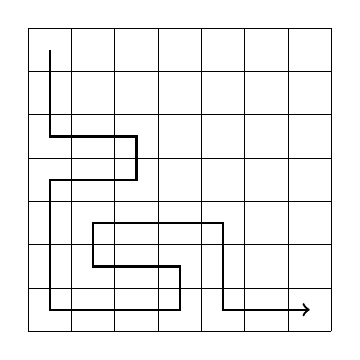
\begin{tikzpicture}[scale=.55]
  \begin{scope}
    \draw (0, 0) grid (7, 7);
    \draw[thick,->] (0.5,6.5) -- (0.5,4.5) -- (2.5,4.5) --
          (2.5,3.5) -- (0.5,3.5) -- (0.5,0.5) --
          (3.5,0.5) -- (3.5,1.5) -- (1.5,1.5) --
          (1.5,2.5) -- (4.5,2.5) -- (4.5,0.5) --
          (6.5,0.5);
  \end{scope}
\end{tikzpicture}
\end{center}
Usando questa osservazione si può terminare la ricerca immediatamente 
quando viene raggiunto l'angolo in basso a destra, risparmiando una 
serie di ulteriori passaggi inutili.

\begin{itemize}
\item
tempo di esecuzione: 119 secondi
\item
numero di chiamate ricorsive: 20 miliardi
\end{itemize}

\subsubsection{Ottimizzazione 3}

Se il percorso tocca uno dei confini esterni e 
può girare a destra o a sinistra, la griglia viene divisa in due parti
che conterrano entrambe quadrati non visitati.
Per esempio nella seguente situazione il percorso può girare sia
a destra che a sinistra:

\begin{center}
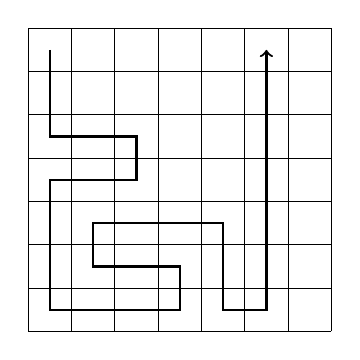
\begin{tikzpicture}[scale=.55]
  \begin{scope}
    \draw (0, 0) grid (7, 7);
    \draw[thick,->] (0.5,6.5) -- (0.5,4.5) -- (2.5,4.5) --
          (2.5,3.5) -- (0.5,3.5) -- (0.5,0.5) --
          (3.5,0.5) -- (3.5,1.5) -- (1.5,1.5) --
          (1.5,2.5) -- (4.5,2.5) -- (4.5,0.5) --
          (5.5,0.5) -- (5.5,6.5);
  \end{scope}
\end{tikzpicture}
\end{center}
In questo caso non è poi più possibile
visitare tutti i quadrati rimanenti e quindi 
la ricerca può essere terminata.
Questa ottimizzazione è molto vantaggiosa:

\begin{itemize}
\item
tempo di esecuzione: 1.8 secondi
\item
numero di chiamate ricorsive: 221 milioni
\end{itemize}

\subsubsection{Ottimizzazione 4}

L'idea dell'Ottimizzazione 3
può essere generalizzata:
se un percorso non può continuare diritto
ma può girare sia a destra che a sinistra,
la griglia si dividerà in due parti entrambe
contenenti quadrati non visitati.
Per esempio si consideri il seguente percorso:

\begin{center}
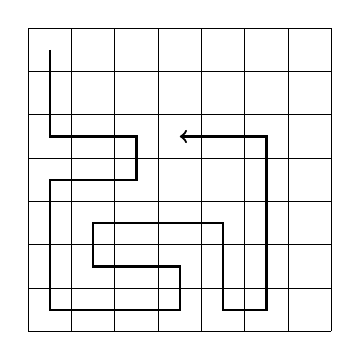
\begin{tikzpicture}[scale=.55]
  \begin{scope}
    \draw (0, 0) grid (7, 7);
    \draw[thick,->] (0.5,6.5) -- (0.5,4.5) -- (2.5,4.5) --
          (2.5,3.5) -- (0.5,3.5) -- (0.5,0.5) --
          (3.5,0.5) -- (3.5,1.5) -- (1.5,1.5) --
          (1.5,2.5) -- (4.5,2.5) -- (4.5,0.5) --
          (5.5,0.5) -- (5.5,4.5) -- (3.5,4.5);
  \end{scope}
\end{tikzpicture}
\end{center}
Risulta chiaro come non sia più possibile visitare tutti i quadrati,
così si può terminare la ricerca.
Dopo quest'ultima ottimizzazione la ricerca risulta molto efficiente:

\begin{itemize}
\item
tempo di esecuzione: 0.6 secondi
\item
numero di chiamate ricorsive: 69 milioni
\end{itemize}

~\\
Dopo aver visto tutte queste ottimizzazioni
si può vedere cosa è stato raggiunto: il
tempo di esecuzione dell'algoritmo originale era di
483 secondi e dopo tutte le ottimizzazioni è diventato di
solo 0,6 secondi. Quindi l'algoritmo è diventato circa 
1000 volte più veloce dopo aver applicato tutte le ottimizzazioni.

Questo succede spesso nel backtracking,
perchè di solito l'albero di ricerca è molto
largo e anche delle semplici osservazioni
possono ridurre drasticamente il tempo di ricerca,
potando molte strade inutili.
Le ottimizzazioni più utili sono quelle che avvengono 
nei primi passaggi dell'algoritmo, cioà nella parte alta 
dell'albero di ricerca.

\section{Meet in the middle}

\index{meet in the middle}

\key{Meet in the middle} is a technique
where the search space is divided into
two parts of about equal size.
A separate search is performed
for both of the parts,
and finally the results of the searches are combined.

The technique can be used
if there is an efficient way to combine the
results of the searches.
In such a situation, the two searches may require less
time than one large search.
Typically, we can turn a factor of $2^n$
into a factor of $2^{n/2}$ using the meet in the
middle technique.

As an example, consider a problem where
we are given a list of $n$ numbers and
a number $x$,
and we want to find out if it is possible
to choose some numbers from the list so that
their sum is $x$.
For example, given the list $[2,4,5,9]$ and $x=15$,
we can choose the numbers $[2,4,9]$ to get $2+4+9=15$.
However, if $x=10$ for the same list,
it is not possible to form the sum.

A simple algorithm to the problem is to
go through all subsets of the elements and
check if the sum of any of the subsets is $x$.
The running time of such an algorithm is $O(2^n)$,
because there are $2^n$ subsets.
However, using the meet in the middle technique,
we can achieve a more efficient $O(2^{n/2})$ time algorithm\footnote{This
idea was introduced in 1974 by E. Horowitz and S. Sahni \cite{hor74}.}.
Note that $O(2^n)$ and $O(2^{n/2})$ are different
complexities because $2^{n/2}$ equals $\sqrt{2^n}$.

The idea is to divide the list into
two lists $A$ and $B$ such that both
lists contain about half of the numbers.
The first search generates all subsets
of $A$ and stores their sums to a list $S_A$.
Correspondingly, the second search creates
a list $S_B$ from $B$.
After this, it suffices to check if it is possible
to choose one element from $S_A$ and another
element from $S_B$ such that their sum is $x$.
This is possible exactly when there is a way to
form the sum $x$ using the numbers of the original list.

For example, suppose that the list is $[2,4,5,9]$ and $x=15$.
First, we divide the list into $A=[2,4]$ and $B=[5,9]$.
After this, we create lists
$S_A=[0,2,4,6]$ and $S_B=[0,5,9,14]$.
In this case, the sum $x=15$ is possible to form,
because $S_A$ contains the sum $6$,
$S_B$ contains the sum $9$, and $6+9=15$.
This corresponds to the solution $[2,4,9]$.

The time complexity of the algorithm is $O(2^{n/2})$,
because both lists $A$ and $B$ contain about $n/2$ numbers
and it takes $O(2^{n/2})$ time to calculate the sums of
their subsets to lists $S_A$ and $S_B$.
After this, it is possible to check in 
$O(2^{n/2})$ time if the sum $x$ can be created
from $S_A$ and $S_B$.